% Nome do capítulo
\chapter{O ambiente Node.Js}
% Label para referenciar
\label{ambiente-node-js}

% Diminuir espaçamento entre título e texto
\vspace{-1.9cm}

% Texto do capítulo

  O Node.Js pode prover um ambiente de programação amplo e forte para os desenvolvedores. Esta pequena introdução
  tem como objetivo resumir o potencial do ambiente em poucos parágrafos.
  
  
  Primeiramente, o JavaScript é uma das linguagens de programação mais utilizadas em interfaces de sites, e o Node.Js
  permite utilizar essa linguagem de programação e aplicá-la em outros contextos como servidores web. Possui um alto
  desempenho através do JavaScript Enginie V8, do Google.\cite{Hughes:2012}.
  
  O V8 utiliza umas das técnicas recentes de compiladores que permite que o código escrito em linguagem de alto nível,
  tal como o JavaScript, execute de forma semelhante a linguagens de baixo nível como C. O Node.Js também aproveita
  do paradigma de orientação a eventos da linguagem e retira proveito disso para produzir servidores escaláveis usando 
  uma arquitetura chamada de ciclo de eventos, do inglês, Event Loop.\cite{Hughes:2012}.
  
  Node.Js é extensível com grandes módulos construídos por uma comunidade ativa desde 2009 quando foi criado
  por Ryan Dhal.
  
\section{Programação Orientada a Eventos}
\label{programacao-orientada-a-eventos}

  O autor \citeonline{Junior:2012} define a programação orientada a eventos, como um paradigma de programação, onde
  pode-se controlar o fluxo da aplicação através de eventos; Um evento indica que algo aconteceu. 
  Em servidores web convencionais, o modelo padrão é o conceito de ação e resposta. 
  O cliente passa a realizar uma requisição a um servidor e aplicação que recebe esta requisição produz uma resposta. 
  O paradigma orientado a eventos utiliza a termonologia de produtor do evento (\textit{event producer}) 
  e o consumidor do evento (\textit{event consumer}).

  \citeonline{Pereira:2013} compara que o Node.Js orientado a eventos se espelha na filosofia de orientação 
  a eventos utilizado pelo JavaScript nos navegadores; a diferença entre eles é que no Node.Js 
  não existe eventos de clique do mouse, teclas pressionadas do teclado (keyup) ou qualquer evento de componentes HTML.
  No Node.Js os eventos trabalhados são entrada e saída do servidor como eventos de conexão 
  ao banco de dados, abertura de arquivo e um dado de um streaming, dentre muitos outros.
  
  A principal diferença em sistemas baseados em evento o produtor do evento não espera pela ação a ser executada
  pelo servidor. \cite{Junior:2012}   


\section{Single thread}
\label{single-thread}

  Single thread em computação pode explicado como a execução de uma única tarefa.
  
  De acordo com \citeonline{Pereira:2013}, em Node.Js nativamente não é possível trabalhar com programação 
  concorrente em plataforma multi-thread, mas existem maneiras de se implementar sistemas concorrentes, 
  como por exemplo, utilizar clusters o qual é um módulo nativo do ambiente Node.Js.
  
  Uma das melhores maneiras para entender o single-thread é descrita por \citeonline{Hughes:2012}
  fazendo uma analogia ao cotidiano de nossa vida.
  
  \citeonline{Hughes:2012} exemplificam que o ser humano é capaz de realizar duas tarefas simples ao mesmo tempo,
  mas que caso uma dessas atividades seja crítica ou grave, ao mesmo tempo, ha chances de algo dar errado muito rapidamente. 
  Isto é como JavaScript. Já que as ações são conduzidas por eventos mas no single-thread apenas uma coisa 
  acontece ao mesmo tempo.
  
  Para \citeonline{Hughes:2012} o conceito single-threaded é muito importante porém é uma das críticas 
  feitas ao Node.Js é a falta de concorrência. Quando \citeonline{Hughes:2012} pronunciou falta de concorrência 
  quis dizer que não são utilizadas todas as CPUs de um computador. 
  Segundo estes autores o problema de executar códigos em várias CPUs de uma vez é que ele requer 
  uma coordenação entre várias "linhas" de execução. Para que várias CPUs possam dividir de maneira eficaz o trabalho, 
  é necessário que eles conversem entre si sobre o estado atual do programa, e o que cada single thread havia feito.
  
  
  Além disso, é possível compartilhar sockets entre processos através da biblioteca multi-node \citeonline{Zyp:2010},
  sendo assim, pode-se ter múltiplos nós de servidores de processos trabalhando em paralelo, 
  cada um em core do processador, mas atenndendo ou escutando a mesma porta, assim o próprio sistema operacional
  atua como balanceador de carga.\cite{Junior:2012}
  
  \cite{Powers:2012} cita também o single thread como um dos benefícios do ambiente do Node.Js 
  pois o aplicativo pode ser facilmente escalável uma vez que em um único segmento de execução não ha uma enorme 
  sobrecarga de requisições. Citando o exemplo de seu livro, ao criar uma aplicação em \ac{PHP} semelhante 
  à aplicação Node.Js o usuário veria a mesma página, mas ao visualzia os processos desta aplicação haverá uma 
  diferença.
  
  Este aplicativo \ac{PHP} no servidor web Apache, cada pedido que for solicitado irá abrir um 
  processo filho do Apache. Em servidores menos otimizados a capacidade de criar processos filhos
  restringe-se a par de centenas de processos filhos em paralelo. Se a por ventura a quantidade de solicitações
  for maior que capacidade de processos filhos do Apache, o cliente entrará numa fila e esperar por uma resposta.\cite{Powers:2012}
  
  Deste modo, um servidor Node.js pode suportar dezenas de milhares de conexões simultâneas, 
  pois ele altera todo o contexto do servidor e o único gargalo passa a ser a capacidade de tráfego 
  de um sistema e não mais o número de conexões.\cite{Abernethy:2011}
  
\section{Chamdas de retorno e \textit{callback's hell}}
\label{chamadas-de-retorno-e-callback-hell}

  De acordo com \citeonline{Wilson:2013} o JavaScript utiliza de \textit{callbacks}
  para abordar o problema a  partir do lado oposto; ao invés de gerenciar processos de execução prolongada, 
  os desenvolvedores associam eventos específicos e escrevem funções especiais, chamadas \textit{callbacks}
  (chamadas de retorno), que são executadas quando o critério do evento é atingido.

\subsection{Evitando \textit{callbacks hell}}

  \cite{Pereira:2013} relata que o JavaScript possui boa performance trabalhando de forma assíncrona porém em certos 
  momentos do desenvolvimentos, inevitavelmente será implementado diversas funções assíncronas encadeadas umas nas 
  outras através das suas funções \textit{callbacks} criando o \textit{callbacks hell}.
  
  No código \ref{leitura-arquivos-diretorio-node} implementado por \citeonline{Pereira:2013}, e referenciado no Anexo \ref{primeiro-anexo}
  ha uma simples leitura de arquivos de um diretório qualquer sendo impresso o nome do arquivo e seu tamanho em
  bytes. Este exemplo feito pelo autor demonstra que uma simples tarefa possui várias chamadas de retorno encadeadas. Também
  é questionado como seria a organização caso a solução do problema fosse mais complexa. Pode-se entender que tal código
  seria um caos e de difícil manutenabilidade.
  
  Também é afirmado, que, a linguagem JavaScript ser assíncrona resulta em ganhos de 
  performace, ha o problema de perda de controle do que está sendo executado, acesso à variáveis devido à troca de escopos
  neste emaranhado de chamadas de retorno.
  
  Um ponto a se atentar, é que, que as chamadas de retorno no Node.Js possuem como parâmetro uma variável de erro. Se existir
  este parâmetro, é recomendado por \citeonline{Pereira:2013} que realize primeiramente o tratamento deste erro na execução da função
  impossibilitando a execução aleatória quando surgir tal erro.
  
  Uma das maneiras de se evitar o temido \textit{callback hell}, e dado que é, uma boa prática de codificação JavaScript é
  criar funções que expressem seu objetivo de forma isoladas, salvando os retornos em váriaveis e passando-as em outros
  chamadas de retorno como parâmetros. A organização do código pode ser visto no código \ref{leitura-arquivos-diretorio-node-callback-heaven} do
  Anexo \ref{primeiro-anexo}.\cite{Pereira:2013}
 
  
  Uma abordagem utilizada pela empresa StrongLoop é a utilização do módulo async \footnote{https://github.com/caolan/async},
  sendo o mais popular entre os desenvolvedores e também fica mais próximo do \textit{core} (núcleo) do Node.Js. Este módulo
  possui o metódo async.waterfall que provê um controle em série, em que os dados podem ser passados para a próxima função
  usando o parametro next. O metódo async.map executa o comando fs.stat (buscar status do arquivo) do Node.Js sobre uma matriz
  de caminhos, em paralelo. Em seguida retorna uma matriz com a ordem mantida dos resultados. Como dito pela empresa
  Strongloop, este módulo garante que somente uma chamada de retorno será retornada, propagação de erros e controle do 
  paralelismo automáticamente. 
  
  Outro módulo é apresentado pela empresa Strongloop é utilização de \textit{Promises} que fornece tratamento de erros
  e regalias de programação funcional. Para tal, é necessário utilizar o módulo Q \footnote{https://github.com/kriskowal/q}
  que através do metódo q.all executa todas as chamadas de status dos arquivos em paralelo e em seguida retorna uma matriz
  com a ordem dos dados mantidas. Ao contrário de exemplos anteriores, quaisquer exceção é lançada dentro da cadeia dos
  \textit{promises}. Somente depois tais exceções são capturadas e manipuladas.
  
  Por fim como descreve a \citeonline{Strongloop:2013} existe a abordagem utilizando \textit{generators} que estarão
  contemplatos e integrados oficialmente em versões posteriores à 0.11.2 do Node.Js. Os \textit{generators} podem ser definidos
  como co-rotinas leves para o JavaScript. Estes \textit{generators} permitem que uma função possa ser suspensa e retornada
  utilizando a palavra reservada yield. A empresa recomenda utilizar o módulo CO \footnote{https://github.com/visionmedia/co},
  mas nada impede a utilização de outros módulos. Ao utilizar o módulo CO é possível manipular erros (incluindo exceções levantadas)
  serão passadas para a função de chamada de retorno. Também é habilitado o uso de blocos \textit{try/catch} em torno das 
  declarações yield.
  
  A empresa \cite{Strongloop:2013} investigou três possibilidades de mitigar o problema dos \textit{callbacks hell}, com o 
  intuito de obtenção de controle do fluxo da aplicação. Um interesse maior surgiu pela a abordagem dos \textit{generators}
  apesar de não empregar em seus projetos. Independente de qual módulo e abordagem for utilizada ela reafirma que é recomendado
  utilizar a modularização em qualquer parte da aplicação e bibliotecas descritas (\textit{async,promises, generators}).
  
  Todo os código e comentários podem ser vistos no artigo da empresa. \cite{Strongloop:2013}
  
\section{Ciclo de eventos}
\label{ciclo-de-eventos}
  
  Ao introduzir esse assunto \cite{Pereira:2013} diz que o ciclo de eventos - Event-Loop - 
  é o agente responsável por escutar e emitir eventos dentro do sistema. Rapidamente explica a teoria do paradigma 
  de orientação a eventos onde o ciclo de eventos é uma repetição infinita que a cada interação verifica em sua 
  fila de eventos se um determinado evento foi emitido ou se existem novos eventos. Estes eventos só aparecem na 
  fila quando são emitidos durante as suas interações na aplicação; quando ocorre, é emitido um evento, então este evento 
  é executado e enviados para a fila de executados.
  
  \cite{Wilson:2013} enaltece os eventos como sendo a alma do Node.Js e do JavaScript. 
  Complementando afirma-se que outras linguagens de programação lidam com fluxos de trabalho em threads múltiplas 
  e concorrentes, com cada thread gastando a maioria de seu tempo aguardando operações bloqueadoras de entrada e 
  saída como leitura ou escrita em disco, manipulação do banco de dados ou acesso a informações pela rede.
  
  \begin{figure}[H]
  % Alterar espaçamentos antes e depois do caption
  \setlength{\abovecaptionskip}{0pt}
  \setlength{\belowcaptionskip}{0pt}
  % Caption
  \caption[Ciclo de eventos no Node.Js]{Ciclo de eventos no Node.Js}
  \centering
  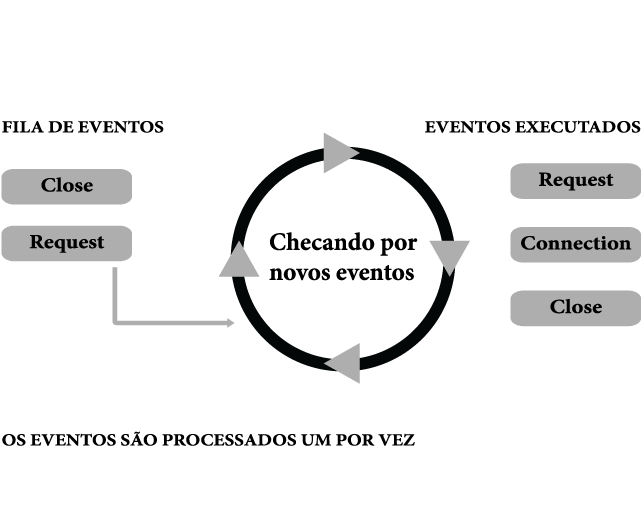
\includegraphics[width=.85\textwidth]{imagem/event-loop-caio-ribeiro.png}
  % Caption centralizada
  \captionsetup{justification=centering}
  \captionfont{\small{\textbf{\\Fonte: \cite{Pereira:2013}}}}	
  \label{fig:event-loop}
  \end{figure}
  
  A figura \ref{fig:event-loop} mostra o ciclo de eventos executado em uma repetição, recebendo o evento \textit{request}.
  
  \cite{Wilson:2013} escreve uma das qualidades do JavaScript, que foi criado seguindo o modelo de programação orientado 
  a eventos. Sendo desde um simples clique de mouse, carregamento de páginas ou envio de formulários, todos utilizando 
  o modelo baseado em eventos.
  
  O \textit{event loop} (cilo de eventos) é o sistema que usa o JavaScript para lidar com os pedidos recebidos de várias
  partes do sistema de uma forma sadia. Há uma série de maneiras como as pessoas lidam com o tempo real ou questões 
  paralelas em computação. 

  
  O JavaScript tem uma abordagem simples que torna o processo muito mais compreensível, mas introduz algumas restrições. 
  Possuindo uma ideia de como o ciclo de eventos funciona, o desenvolvedor é capaz de usá-lo em toda sua potencialidade, 
  conseguindo vantagens e evitando armadilhas dessa abordagem.\cite{Hughes:2012}
  
  Pensamos que a maioria das pessoas entendem intuitivamente a programação orientada a eventos, porquê é como a 
  vida cotidiana onde cada solicitação de evento necessita de um retorno. A programação orientada a eventos faz a 
  mesma coisa. Ao permitir que o desenvolvedor escreva código que só trabalhe em um retorno de chamada de cada vez, 
  o programa será compreensível e também capaz de executar rapidamente várias tarefas de forma eficiente.\cite{Hughes:2012}
  
  Como apresentado por \cite{Pereira:2013} o EventEmitter, é o módulo responsável por por emitir estes eventos e em 
  grande maioria das bibliotecas do ambiente Node.Js utiliza as funcionalidades de eventos deste módulo. 
  No processo de execução do evento pode-se programar qualquer lógica de programação através do 
  mecanismo de chamada de retorno. Tal chamada de retorno pode ser executado através de uma função de escuta, 
  semanticamente conhecida pelo on().
  
  Essa seção é bem descrita e exemplificada por \cite{Wilson:2013} em seu livro que nos mostra o uso e o 
  desenvolvimento de eventos.

  
  Finalizando o ciclo de eventos seção, \cite{Pereira:2013} diz que a programação orientada a eventos do Node.Js 
  foi inspirado pelos \textit{frameworks} Event Machine\footnote{http://rubyeventmachine.com/} do 
  Ruby\footnote{https://www.ruby-lang.org/en/} e Twisted\footnote{https://twistedmatrix.com/trac/} do 
  Python\footnote{https://www.python.org/}, porém o ciclo de eventos do Node.Js é mais perfomático pois seu mecanismo 
  é nativamente executado de forma não bloqueante sendo o diferencial em relação a outros ambientes de programação.
  
\section{Por que usar assíncrono}
\label{porque-usar-assincrono}

  No ambiente de desenvolvimento Node.Js é importante entender e saber trabalhar com as chamadas assíncronas. 
  \cite{Pereira:2013} em seu livro exemplifica em código as diferenças entre uma função síncrona e assíncrona 
  em relação ao tempo em que são executadas. Este código nada mais é que uma repetição de 5 interações e a cada 
  iteração desta repetição será criado um arquivo texto.
  
  Veja o tempo gasto utilizando o modelo síncrono da função \textit{fs.writeFileSync}.
  
  \begin{figure}[H]
  % Alterar espaçamentos antes e depois do caption
  \setlength{\abovecaptionskip}{0pt}
  \setlength{\belowcaptionskip}{0pt}
  % Caption
  \caption[Tempo de resposta, metódo síncrono bloqueante]{Tempo de resposta, metódo síncrono bloqueante}
  \centering
  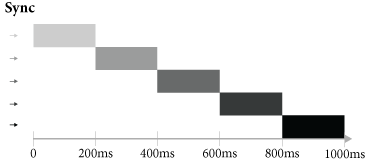
\includegraphics[width=.85\textwidth]{imagem/timeline-node-sync-caio-ribeiro.png}
  % Caption centralizada
  \captionsetup{justification=centering}
  \captionfont{\small{\textbf{\\Fonte: \cite{Pereira:2013}}}}	
  \label{fig:timeline-sync}
  \end{figure}
  
  A Figura \ref{fig:timeline-sync} exibe um quadro com um tempo de 200 ms de resposta para cada um dos 5 arquivos.

  \begin{figure}[H]
  % Alterar espaçamentos antes e depois do caption
  \setlength{\abovecaptionskip}{0pt}
  \setlength{\belowcaptionskip}{0pt}
  % Caption
  \caption[Tempo de resposta, metódo assíncrono não-bloqueante]{Tempo de resposta, metódo assíncrono não-bloqueante}
  \centering
  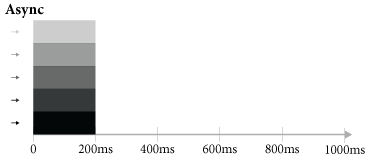
\includegraphics[width=.85\textwidth]{imagem/timeline-node-async-caio-ribeiro.png}
  % Caption centralizada
  \captionsetup{justification=centering}
  \captionfont{\small{\textbf{\\Fonte: \cite{Pereira:2013}}}}	
  \label{fig:timeline-async}
  \end{figure}

  
  Agora na Figura \ref{fig:timeline-async} o tempo total de duração foram de 200 milesegundos, pois foram executados
  de forma assíncrona maximizando o processamento.

\section{Framework Express}
\label{framework-express}

  \cite{Powers:2012} descreve que no geral um \textit{framework} ajuda na infraestrutura e que nos permite criar sites e aplicações
  com agilidade, fornecendo ao desenvolvedor um esqueleto capaz de oferecer um suporte no processo de desenvolvimento de
  software. Com os \textit{frameworks} foca-se na criação de funcionalidades da nossa aplicação ou site e 
  também fornece coesão ao código, o que nos beneficia com legibilidade e manutenabilidade.

  \cite{Pereira:2013} complementa que utilizar a API HTTP nativa do Node.Js pode ser um processo moroso e desgastante
  para o desenvolvedor. 
  Conforme surgem novas necessidades de implementação e novas funcionalidades serão acrescidas,
  os códigos se tornarão gigantescos aumentando a complexidade do projeto e dificultando futuras manutenções.
  
  Assim surge o \textit{framework} Express.Js para solucionar necessidades e agilizar no desenvolvimento.
  
  \citeonline{Powers:2012} compara que o \textit{Express.Js} é parecido com o \textit{framework} Sinatra porém bem mais \textit{RESTFUL}. 
  Pereira(2012) reafirma e complementa que o módulo \textit{Express.Js} foi inspirado pelo \textit{framework} Sinatra da 
  linguagem Ruby e que é bastante utilizado em aplicações web de grande escala.
  
  Suas características são descritas por \citeonline{Pereira:2013}:
  
  \begin{compactitem}
    \item[a)] \ac{MVR};   
    
    \item[b)] \ac{MVC};
    
    \item[c)] Roteamento de \ac{URL} com chamadas de retorno;
    
    \item[d)] Middleware;
    
    \item[e)] Interface \ac{REST};
    
    \item[f)] Suporte a File Uploads.
    
    \item[g)] Configuração baseada em variáveis de ambiente;
    
    \item[h)] Suporte a helpers dinâmicos;
    
    \item[i)] Integração com Templates Enginies;
    
    \item[j)] Integração com SQL e NoSQL;
    
  \end{compactitem}
  
  Ao criar um esqueleto utilizando o \textit{Express.js} é importante ter conhecimento do que cada
  arquivo ou diretório representa. \cite{Powers:2012, Hughes:2012} não apresentam um descritivo de cada arquivo 
  ou diretório e seu papel. Entretanto \cite{Pereira:2013, Wilson:2013} aprofundam mais neste assunto que podem ser vistos
  no \ref{apend:express-skel}.
  
  O arquivo de \textit{package.json}, de acordo com \citeonline{Wilson:2013} sempre é necessário ser criado 
  em seu projeto e que ele é responsável por fornecer detalhes sobre as condições de operação e configuração 
  esperadas por seu código. \cite{Wilson:2013} complementa que este arquivo ajuda a prevenir que alterações 
  futuras em módulos de terceiros quebrem a lógica da aplicação.

  No livro, \cite{Wilson:2013} exibe um exemplo do arquivo 
  \textit{package.json} o qual é utilizado para sincronizar a aplicação com dependências, sendo importante associar 
  a aplicação a uma versão especifica. 
  
  Para maiores detalhes sobre as notações semânticas utilizada pelo \ac{NPM} visite a documentação \cite{Semver:2013}.

\subsection{O servidor web com \textit{Express.Js}}
\label{servidor-web-express-js}

  
  De acordo com \cite{Wilson:2013} o interessante do Node.Js é que o código do 
  programa que se escreve para ele também é a implementação do servidor. 
  Seguindo este modelo tem-se a expectativa de que a aplicação funcione e se comporte de modo semelhante 
  ao ambiente de produção assim como no desenvolvimento, pois não existe nenhuma biblioteca, nenhum intermediário 
  ou \textit{daemon} que esteja no caminho.
  
  O arquivo app.js criado pelo \textit{Express.js} é em suma pequeno mas com grandes funcionalidades inclusas como 
  roteamento para solicitações \ac{HTTP} entrantes, motores de visões para renderizar marcações do HTML5
  e também download dos arquivos estáticos.